\chapter{Conclusion and Discussion}
\setlength{\parindent}{2.5em}
This project presents a helmet and head detection system trained on a custom dataset using the YOLOv8 architecture, combined with a counting mechanism applied to university CCTV footage. The final model achieved significant accuracy improvements in helmet detection, reaching up to 95\% in our latest version. And applying them to the test videos we have detection average of 91.75\% across all classes detection. Looking at counting methods The double-line counting method effectively reduced duplicate counts and stabilized results, especially for slow-moving or occluded objects. For person and motorbike tracking, the system performed well in low-overlap conditions, providing strong results that demonstrate the system’s potential for practical monitoring and analysis of helmet usage compliance. Additionally we were able to obstecle of counting person, as mentioned there were issues regarding the person detection, as for some cases there were children which are unable to be detected by YOLOv8 pretrained models, another instances such as people overlapping when riding the motor bike, for this case we have switched to combine the count of helmet and head together to total the number of persons. This step is important as be can conclude that our helmet and head detection where accurate enough to combine their count as people. Moreover there where also issues regarding flickering detections for motorbike. For this cases where have used the tracker, and allow the system to store the tracker location and ID through track\_history. This function allows us to compare the possition of the previous detection and the new detection. This is to make sure that the tracker rememebers the movement of the object it is tracking. The counting for the motorbike is done solely based on the tracker's center point of the bouding boxes and comparing the ID history position with the current position to help aid with the Bot\_sort Tracker. This method works well with the YOLOv8 pretrained model for motorbike detection, simply we were able to find a Region of Interest so that we do not also count motor bike and people going out of the scene. 


\section{Obstacles}

\begin{center}
	\begin{minipage}{0.45\textwidth}
		\centering
		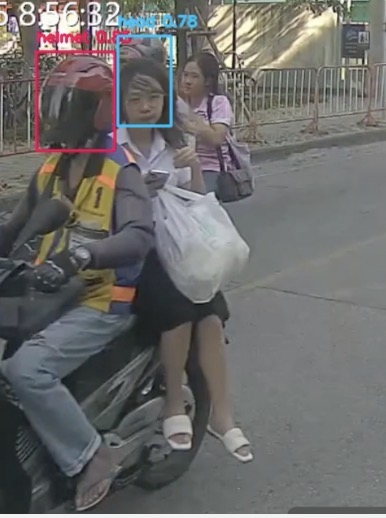
\includegraphics[width=\linewidth]{limitation2.png}
		\vspace{0.5em} % Adjust as needed
		
		\textbf{Figure 5.1}
	\end{minipage}
	\hfill
	\begin{minipage}{0.45\textwidth}
		\centering
		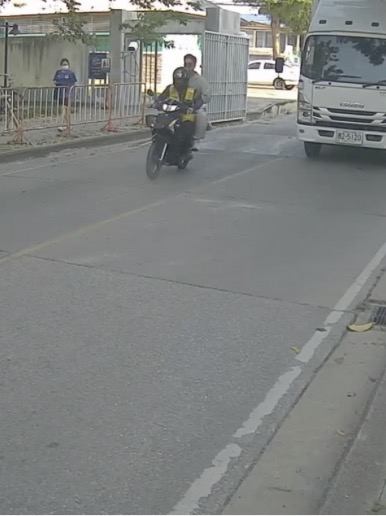
\includegraphics[width=\linewidth]{limitation3.png}
		\vspace{0.5em} % Match the first one
		
		\textbf{Figure 5.2}
	\end{minipage}
\end{center}
\setlength{\parindent}{2.5em}
During system development and testing, the main challenge involved dealing with overlapping bounding boxes, particularly when multiple motorcycles and riders appeared close together. This sometimes led to incorrect object counts or detection errors, such as merging two people into one or misidentifying a detection. The tracking system also struggled when many objects entered the counting zone at once, occasionally creating new IDs for the same object however we uses Bot\_sort Tracker to help minimize the flickering as possible, as when they enter the counting zone, if object is redetected there are chances new ID will appear and our system could not reidentify the object, it would count that object base on the new ID.

 These issues were more pronounced in crowded scenes and highlight the limitations of relying on bounding box-based tracking in complex real-world environments. which can be seen in Figure 5.1. This sometimes led to incorrect object counts or detection errors, because there are another object blocking another object in the counting zone. 

In Figure 5.2 another flaw showing the struggle of tracking system when an object appear to be on another lane, causing it hard for our model to detect an object, especially when it appear to far from the annotation point.


\section{Future Work}
\setlength{\parindent}{2.5em}
In future iterations, the focus will be on improving both the detection model and the tracking accuracy. Training with more diverse and balanced data will help the model generalize better across various environments and video conditions. Further enhancement of the counting and tracking logic is also planned to address issues with ID switching and occlusion. Additionally, while deployment to the university server is not yet complete, it remains a key objective for real-time monitoring in a practical setting. These improvements will support the goal of developing a more accurate, stable, and scalable helmet compliance monitoring system.



